\documentclass[twoside]{book}

% Packages required by doxygen
\usepackage{fixltx2e}
\usepackage{calc}
\usepackage{doxygen}
\usepackage[export]{adjustbox} % also loads graphicx
\usepackage{graphicx}
\usepackage[utf8]{inputenc}
\usepackage{makeidx}
\usepackage{multicol}
\usepackage{multirow}
\PassOptionsToPackage{warn}{textcomp}
\usepackage{textcomp}
\usepackage[nointegrals]{wasysym}
\usepackage[table]{xcolor}

% NLS support packages
\usepackage[brazil]{babel}
% Font selection
\usepackage[T1]{fontenc}
\usepackage[scaled=.90]{helvet}
\usepackage{courier}
\usepackage{amssymb}
\usepackage{sectsty}
\renewcommand{\familydefault}{\sfdefault}
\allsectionsfont{%
  \fontseries{bc}\selectfont%
  \color{darkgray}%
}
\renewcommand{\DoxyLabelFont}{%
  \fontseries{bc}\selectfont%
  \color{darkgray}%
}
\newcommand{\+}{\discretionary{\mbox{\scriptsize$\hookleftarrow$}}{}{}}

% Page & text layout
\usepackage{geometry}
\geometry{%
  a4paper,%
  top=2.5cm,%
  bottom=2.5cm,%
  left=2.5cm,%
  right=2.5cm%
}
\tolerance=750
\hfuzz=15pt
\hbadness=750
\setlength{\emergencystretch}{15pt}
\setlength{\parindent}{0cm}
\setlength{\parskip}{3ex plus 2ex minus 2ex}
\makeatletter
\renewcommand{\paragraph}{%
  \@startsection{paragraph}{4}{0ex}{-1.0ex}{1.0ex}{%
    \normalfont\normalsize\bfseries\SS@parafont%
  }%
}
\renewcommand{\subparagraph}{%
  \@startsection{subparagraph}{5}{0ex}{-1.0ex}{1.0ex}{%
    \normalfont\normalsize\bfseries\SS@subparafont%
  }%
}
\makeatother

% Headers & footers
\usepackage{fancyhdr}
\pagestyle{fancyplain}
\fancyhead[LE]{\fancyplain{}{\bfseries\thepage}}
\fancyhead[CE]{\fancyplain{}{}}
\fancyhead[RE]{\fancyplain{}{\bfseries\leftmark}}
\fancyhead[LO]{\fancyplain{}{\bfseries\rightmark}}
\fancyhead[CO]{\fancyplain{}{}}
\fancyhead[RO]{\fancyplain{}{\bfseries\thepage}}
\fancyfoot[LE]{\fancyplain{}{}}
\fancyfoot[CE]{\fancyplain{}{}}
\fancyfoot[RE]{\fancyplain{}{\bfseries\scriptsize Gerado por Doxygen }}
\fancyfoot[LO]{\fancyplain{}{\bfseries\scriptsize Gerado por Doxygen }}
\fancyfoot[CO]{\fancyplain{}{}}
\fancyfoot[RO]{\fancyplain{}{}}
\renewcommand{\footrulewidth}{0.4pt}
\renewcommand{\chaptermark}[1]{%
  \markboth{#1}{}%
}
\renewcommand{\sectionmark}[1]{%
  \markright{\thesection\ #1}%
}

% Indices & bibliography
\usepackage{natbib}
\usepackage[titles]{tocloft}
\setcounter{tocdepth}{3}
\setcounter{secnumdepth}{5}
\makeindex

% Hyperlinks (required, but should be loaded last)
\usepackage{ifpdf}
\ifpdf
  \usepackage[pdftex,pagebackref=true]{hyperref}
\else
  \usepackage[ps2pdf,pagebackref=true]{hyperref}
\fi
\hypersetup{%
  colorlinks=true,%
  linkcolor=blue,%
  citecolor=blue,%
  unicode%
}

% Custom commands
\newcommand{\clearemptydoublepage}{%
  \newpage{\pagestyle{empty}\cleardoublepage}%
}

\usepackage{caption}
\captionsetup{labelsep=space,justification=centering,font={bf},singlelinecheck=off,skip=4pt,position=top}

%===== C O N T E N T S =====

\begin{document}

% Titlepage & ToC
\hypersetup{pageanchor=false,
             bookmarksnumbered=true,
             pdfencoding=unicode
            }
\pagenumbering{roman}
\begin{titlepage}
\vspace*{7cm}
\begin{center}%
{\Large Projeto Final de Embarcados \\[1ex]\large 1.\+0 }\\
\vspace*{1cm}
{\large Gerado por Doxygen 1.8.11}\\
\end{center}
\end{titlepage}
\clearemptydoublepage
\tableofcontents
\clearemptydoublepage
\pagenumbering{arabic}
\hypersetup{pageanchor=true}

%--- Begin generated contents ---
\chapter{Página Principal}
\label{index}\hypertarget{index}{}\hypertarget{index_intro_sec}{}\section{Descrição}\label{index_intro_sec}
Este projeto foi delegado aos estudantes da turma de Sistemas Embarcados, no período de 2017.\+2, pelo professor da Universidade Federal de Alagoas (U\+Fal) Rodrigo Peixoto. O estudo realizado aqui tem como principal proposta exercitar os conhecimentos aprendidos em sala de aula, referentes aos conceitos e técnicas no que tange o desenvolvimento de e para sistemas embarcados. Desta forma, foi proposto o desenvolvimento de cinco casos de teste, que contemplassem os conceitos aprendidos, anteriormente mencionados, e as funcionalidades presentes na placa utilizada, a Micro\+Bit. Os cinco casos de teste consistiam em\+:
\begin{DoxyItemize}
\item Caso 01\+: Mostrar o texto \char`\"{}\+E\+C\+O\+M042.\+2017.\+2\char`\"{} no display de forma que ele fique passando no display.
\item Caso 02\+: Deve utilizar o acelerômetro para movimentar um ponto (apenas um led da matriz) que dependendo da posição da placa ele vai se mover;
\item Caso 03\+: Deve utilizar a bússola para mostrar onde está o norte magnético. Essa indicação deve ser feita na matriz de leds;
\item Caso 04\+: Mostrar a temperatura capturada pelo sensor da placa em graus célsius;
\item Caso 05\+: Deve utilizar o bluetooth para interagir com um aparelho externo (ex. celular ou computador) deve trocar dados nessa interação. Fica a critério do aluno definir como mostrar que a troca de dados ocorre de forma correta. Dica, pode mostrar na matriz de led o valor passado pelo outro computador.
\end{DoxyItemize}

Onde somente quatro se fizeram possíveis de serem implementados.\hypertarget{index_install_sec}{}\section{Execução do Projeto}\label{index_install_sec}
Para execução do projeto desenvolvido para este projeto, deve-\/se baixá-\/lo do repositório online e instalar algumas depedências\+: 
\begin{DoxyCode}
1 sudo apt-get install putty
2 git clone https://github.com/BrunoGeorgevich/EmbbededSystemsProject
\end{DoxyCode}


Logo em seguida, deve-\/se entrar no diretório baixado, através do comando\+: 
\begin{DoxyCode}
1 cd EmbbededSystemsProject
\end{DoxyCode}


Para que então se possa compilar e gerar o binário referente a Micro\+Bit\+: 
\begin{DoxyCode}
1 cd build
2 cmake ..
3 make -j7
\end{DoxyCode}


Caso todo o processo de compilação e geração tenha dado certo, agora basta copiar o binário gerado e copiá-\/lo para a Micro\+Bit\+: 
\begin{DoxyCode}
1 cp zephyr/zephyr.bin [CAMINHO PARA A SUA MICROBIT]
\end{DoxyCode}


Tendo copiado o binário para a Micro\+Bit a mesma irá reiniciar e desconectar do computador. Logo após ela automaticamente reconectar, execute a linha de comando abaixo para comunicar-\/se com ela via serial\+: 
\begin{DoxyCode}
1 sudo putty /dev/ttyACM0 -serial -sercfg 115200,8,n,1,N
\end{DoxyCode}


Para gerar a documentação para o mesmo, deve-\/se executar as seguites linhas de código\+: 
\begin{DoxyCode}
1 cd ../src/ && doxygen dox\_config
\end{DoxyCode}
 
\chapter{Índice das Estruturas de Dados}
\section{Estruturas de Dados}
Aqui estão as estruturas de dados, uniões e suas respectivas descrições\+:\begin{DoxyCompactList}
\item\contentsline{section}{\hyperlink{structi2c__dev}{i2c\+\_\+dev} }{\pageref{structi2c__dev}}{}
\item\contentsline{section}{\hyperlink{structstate}{state} \\*Struct que modela o formato de um estado da Máquina de Estados }{\pageref{structstate}}{}
\end{DoxyCompactList}

\chapter{Índice dos Arquivos}
\section{Lista de Arquivos}
Esta é a lista de todos os arquivos documentados e suas respectivas descrições\+:\begin{DoxyCompactList}
\item\contentsline{section}{\hyperlink{accelerometer_8h}{accelerometer.\+h} \\*Este arquivo contém as funções, constantes e variáveis relacionadas a funcionalidade do Acelerômetro }{\pageref{accelerometer_8h}}{}
\item\contentsline{section}{\hyperlink{compass_8h}{compass.\+h} \\*Este arquivo contém as funções, constantes e variáveis relacionadas a funcionalidade da Bússola }{\pageref{compass_8h}}{}
\item\contentsline{section}{\hyperlink{configure_8h}{configure.\+h} \\*Este arquivo contém as funções, constantes e variáveis responsáveis por configurar e abstrair os Sensores da Micro\+Bit }{\pageref{configure_8h}}{}
\item\contentsline{section}{\hyperlink{helloworld_8h}{helloworld.\+h} \\*Este arquivo contém as funções, constantes e variáveis relacionadas a funcionalidade Hello\+World }{\pageref{helloworld_8h}}{}
\item\contentsline{section}{\hyperlink{i2c__utils_8h}{i2c\+\_\+utils.\+h} \\*Este arquivo contém as constantes, funções e variáveis relacionadas a Comunicação I²C }{\pageref{i2c__utils_8h}}{}
\item\contentsline{section}{\hyperlink{includes_8h}{includes.\+h} \\*Este arquivo contém todas as bibliotecas necessárias para os arquivos .h }{\pageref{includes_8h}}{}
\item\contentsline{section}{\hyperlink{state_8h}{state.\+h} \\*Este arquivo contém as constantes e variáveis relacionadas a Máquina de Estados }{\pageref{state_8h}}{}
\item\contentsline{section}{\hyperlink{temperature_8h}{temperature.\+h} \\*Este arquivo contém as funções, constantes e variáveis relacionadas a funcionalidade do Sensor de Temperatura }{\pageref{temperature_8h}}{}
\end{DoxyCompactList}

\chapter{Estruturas}
\hypertarget{structi2c__dev}{}\section{Referência da Estrutura i2c\+\_\+dev}
\label{structi2c__dev}\index{i2c\+\_\+dev@{i2c\+\_\+dev}}
\subsection*{Campos de Dados}
\begin{DoxyCompactItemize}
\item 
struct device $\ast$ {\bfseries dev}\hypertarget{structi2c__dev_ac4b6ba60143ff90df0ddc847deed7499}{}\label{structi2c__dev_ac4b6ba60143ff90df0ddc847deed7499}

\item 
char {\bfseries name} \mbox{[}I2\+C\+\_\+\+D\+E\+V\+I\+C\+E\+\_\+\+N\+A\+M\+E\+\_\+\+L\+E\+N\+G\+TH\mbox{]}\hypertarget{structi2c__dev_aa3e3ecd39bec0681b174122b4a5e91e5}{}\label{structi2c__dev_aa3e3ecd39bec0681b174122b4a5e91e5}

\item 
u16\+\_\+t {\bfseries addr}\hypertarget{structi2c__dev_ae9308c72bfb06fea21da16f47b4e679b}{}\label{structi2c__dev_ae9308c72bfb06fea21da16f47b4e679b}

\item 
u8\+\_\+t {\bfseries reg\+\_\+test}\hypertarget{structi2c__dev_a20bd6a8e30216a5866cfc70fec9a3203}{}\label{structi2c__dev_a20bd6a8e30216a5866cfc70fec9a3203}

\item 
u8\+\_\+t {\bfseries reg\+\_\+test\+\_\+expected\+\_\+val}\hypertarget{structi2c__dev_a46e0fffcf23e10012b1f5afc774088e7}{}\label{structi2c__dev_a46e0fffcf23e10012b1f5afc774088e7}

\end{DoxyCompactItemize}


A documentação para esta estrutura foi gerada a partir do seguinte arquivo\+:\begin{DoxyCompactItemize}
\item 
\hyperlink{i2c__utils_8h}{i2c\+\_\+utils.\+h}\end{DoxyCompactItemize}

\hypertarget{structstate}{}\section{Referência da Estrutura state}
\label{structstate}\index{state@{state}}


Struct que modela o formato de um estado da Máquina de Estados.  




{\ttfamily \#include $<$state.\+h$>$}

\subsection*{Campos de Dados}
\begin{DoxyCompactItemize}
\item 
\begin{tabbing}
xx\=xx\=xx\=xx\=xx\=xx\=xx\=xx\=xx\=\kill
union \{\\
\>struct {\bfseries internal\_states} \{\\
\>\>enum \hyperlink{state_8h_aa0aafed44fec19806d8f9ad834be1248}{state\_t} \hyperlink{structstate_a276d20af15eb7cc14800557d670eb8a5}{previous}\\
\>\>enum \hyperlink{state_8h_aa0aafed44fec19806d8f9ad834be1248}{state\_t} \hyperlink{structstate_aa23ac3f3183e79172bab91684e0195e1}{current}\\
\>\>enum \hyperlink{state_8h_aa0aafed44fec19806d8f9ad834be1248}{state\_t} \hyperlink{structstate_a24e4d9ff5dc7891e048ee578ba970837}{next}\\
\>\} \hypertarget{unionstate_1_1_0D0_a3c849dbd83637b100181b78ad752620c}{}\label{unionstate_1_1_0D0_a3c849dbd83637b100181b78ad752620c}
\\
\>enum \hyperlink{state_8h_aa0aafed44fec19806d8f9ad834be1248}{state\_t} \hyperlink{structstate_a8a9de0cd847e8ae900e15eb66fe408f2}{s} \mbox{[}3\mbox{]}\\
\}; \hypertarget{structstate_a836fa023107dfb286044c007f23358b7}{}\label{structstate_a836fa023107dfb286044c007f23358b7}
\\

\end{tabbing}\item 
void($\ast$ \hyperlink{structstate_a90aac7b165377e812886e60e28d054bf}{run} )(void)
\end{DoxyCompactItemize}


\subsection{Descrição Detalhada}
Struct que modela o formato de um estado da Máquina de Estados. 

\subsection{Campos}
\index{state@{state}!current@{current}}
\index{current@{current}!state@{state}}
\subsubsection[{\texorpdfstring{current}{current}}]{\setlength{\rightskip}{0pt plus 5cm}enum {\bf state\+\_\+t} state\+::current}\hypertarget{structstate_aa23ac3f3183e79172bab91684e0195e1}{}\label{structstate_aa23ac3f3183e79172bab91684e0195e1}
Referencia o estado atual \index{state@{state}!next@{next}}
\index{next@{next}!state@{state}}
\subsubsection[{\texorpdfstring{next}{next}}]{\setlength{\rightskip}{0pt plus 5cm}enum {\bf state\+\_\+t} state\+::next}\hypertarget{structstate_a24e4d9ff5dc7891e048ee578ba970837}{}\label{structstate_a24e4d9ff5dc7891e048ee578ba970837}
Referencia o estado posterior \index{state@{state}!previous@{previous}}
\index{previous@{previous}!state@{state}}
\subsubsection[{\texorpdfstring{previous}{previous}}]{\setlength{\rightskip}{0pt plus 5cm}enum {\bf state\+\_\+t} state\+::previous}\hypertarget{structstate_a276d20af15eb7cc14800557d670eb8a5}{}\label{structstate_a276d20af15eb7cc14800557d670eb8a5}
$<$ Referencia os estado anterior, atual e posterior Referencia o estado anterior \index{state@{state}!run@{run}}
\index{run@{run}!state@{state}}
\subsubsection[{\texorpdfstring{run}{run}}]{\setlength{\rightskip}{0pt plus 5cm}void($\ast$ state\+::run) (void)}\hypertarget{structstate_a90aac7b165377e812886e60e28d054bf}{}\label{structstate_a90aac7b165377e812886e60e28d054bf}
Referencia o método a ser executado pelo estado atual \index{state@{state}!s@{s}}
\index{s@{s}!state@{state}}
\subsubsection[{\texorpdfstring{s}{s}}]{\setlength{\rightskip}{0pt plus 5cm}enum {\bf state\+\_\+t} state\+::s\mbox{[}3\mbox{]}}\hypertarget{structstate_a8a9de0cd847e8ae900e15eb66fe408f2}{}\label{structstate_a8a9de0cd847e8ae900e15eb66fe408f2}
Permite o acesso às referencias dos estados por um Array 

A documentação para esta estrutura foi gerada a partir do seguinte arquivo\+:\begin{DoxyCompactItemize}
\item 
\hyperlink{state_8h}{state.\+h}\end{DoxyCompactItemize}

\chapter{Arquivos}
\hypertarget{accelerometer_8h}{}\section{Referência do Arquivo accelerometer.\+h}
\label{accelerometer_8h}\index{accelerometer.\+h@{accelerometer.\+h}}


Este arquivo contém as funções, constantes e variáveis relacionadas a funcionalidade do Acelerômetro.  


{\ttfamily \#include \char`\"{}includes.\+h\char`\"{}}\\*
Gráfico de dependência de inclusões para accelerometer.\+h\+:\nopagebreak
\begin{figure}[H]
\begin{center}
\leavevmode
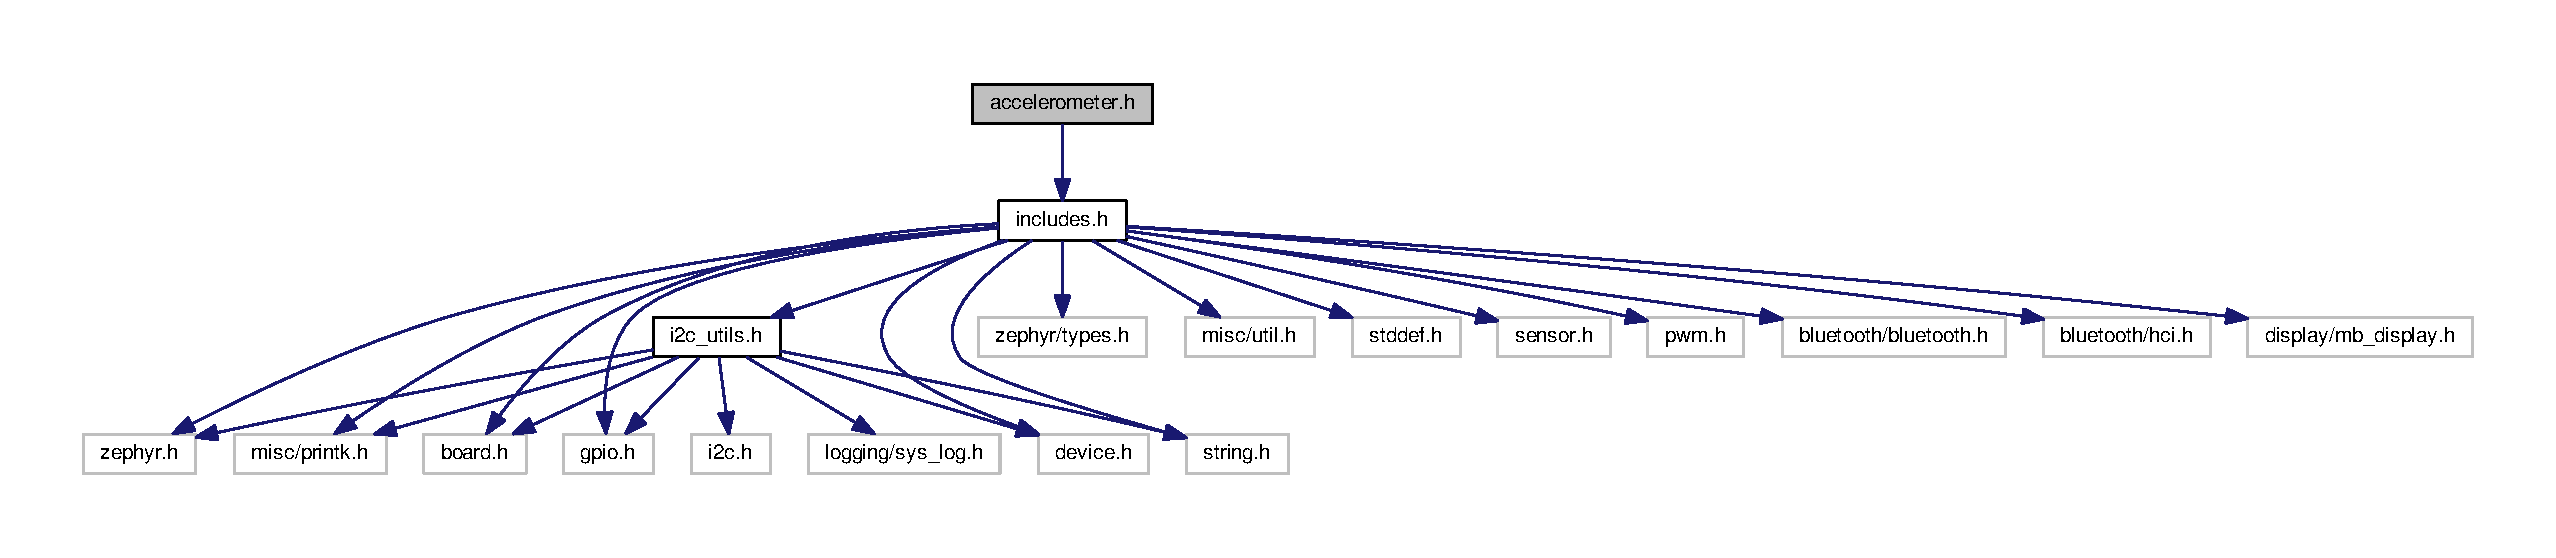
\includegraphics[width=350pt]{accelerometer_8h__incl}
\end{center}
\end{figure}
Este grafo mostra quais arquivos estão direta ou indiretamente relacionados com este arquivo\+:\nopagebreak
\begin{figure}[H]
\begin{center}
\leavevmode
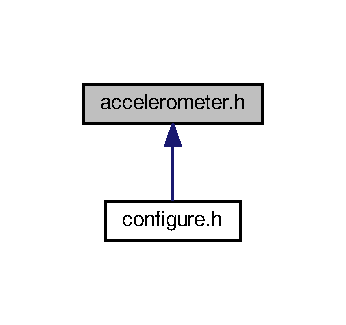
\includegraphics[width=166pt]{accelerometer_8h__dep__incl}
\end{center}
\end{figure}
\subsection*{Definições e Macros}
\begin{DoxyCompactItemize}
\item 
\#define \hyperlink{accelerometer_8h_a58ef4e483804701597e8f9d4fa71bfba}{A\+C\+C\+E\+L\+E\+R\+O\+M\+E\+T\+E\+R\+\_\+\+A\+D\+D\+R\+E\+SS}~0x1D
\item 
\#define \hyperlink{accelerometer_8h_a622bb7a97158370bf70d07a7522ab0bc}{A\+C\+C\+E\+L\+E\+R\+O\+M\+E\+T\+E\+R\+\_\+\+R\+E\+G\+I\+S\+T\+ER}~0x0D
\item 
\#define \hyperlink{accelerometer_8h_a3846d9aa5bacabceb64cd0ba1e7c7d07}{A\+C\+C\+E\+L\+E\+R\+O\+M\+E\+T\+E\+R\+\_\+\+T\+E\+ST}~0x5A
\item 
\#define \hyperlink{accelerometer_8h_adace40e77aaef2412bae491e9120ff29}{R\+E\+F\+R\+E\+S\+H\+\_\+\+T\+I\+M\+E\+\_\+\+A\+C\+C\+E\+L\+E\+R\+O\+M\+E\+T\+ER}~16
\end{DoxyCompactItemize}
\subsection*{Funções}
\begin{DoxyCompactItemize}
\item 
int \hyperlink{accelerometer_8h_a0796c8d57cbb60c0d2c2aa1558124ac5}{translate\+\_\+pos\+\_\+accelerometer} (int32\+\_\+t val)
\begin{DoxyCompactList}\small\item\em Função que traduz os valores coletados pelo Acelerômetro para uma posição em uma Matriz 5x5. \end{DoxyCompactList}\item 
void \hyperlink{accelerometer_8h_a7ac739d7e94d1b44dfde2fd32f049285}{accelerometer\+\_\+display} (int32\+\_\+t x, int32\+\_\+t y)
\begin{DoxyCompactList}\small\item\em Função que irá representar a variação do Acelerômetro em uma Matriz 5x5. \end{DoxyCompactList}\item 
void \hyperlink{accelerometer_8h_a70c79e23dab9678c5653ccedbb9c500e}{accelerometer\+\_\+showcase} ()\hypertarget{accelerometer_8h_a70c79e23dab9678c5653ccedbb9c500e}{}\label{accelerometer_8h_a70c79e23dab9678c5653ccedbb9c500e}

\begin{DoxyCompactList}\small\item\em Função que irá executar a funcionalidade do Acelerômetro Implementada. \end{DoxyCompactList}\item 
void \hyperlink{accelerometer_8h_aedd212ed9cb67e88387fee6a77e97187}{init\+\_\+accelerometer} ()\hypertarget{accelerometer_8h_aedd212ed9cb67e88387fee6a77e97187}{}\label{accelerometer_8h_aedd212ed9cb67e88387fee6a77e97187}

\begin{DoxyCompactList}\small\item\em Função que irá iniciar as variáveis responsáveis pelo bom funcionamento do Acelerômetro. \end{DoxyCompactList}\end{DoxyCompactItemize}
\subsection*{Variáveis}
\begin{DoxyCompactItemize}
\item 
struct \hyperlink{structi2c__dev}{i2c\+\_\+dev} \hyperlink{accelerometer_8h_ac62d82f0fd3bae2affcd081de51f4301}{accelerometer}\hypertarget{accelerometer_8h_ac62d82f0fd3bae2affcd081de51f4301}{}\label{accelerometer_8h_ac62d82f0fd3bae2affcd081de51f4301}

\begin{DoxyCompactList}\small\item\em Variável responsável por estabelecer a comunicação I²C com o Acelerômetro. \end{DoxyCompactList}\end{DoxyCompactItemize}


\subsection{Descrição Detalhada}
Este arquivo contém as funções, constantes e variáveis relacionadas a funcionalidade do Acelerômetro. 

\begin{DoxyAuthor}{Autor}
Bruno Georgevich Ferreira 
\end{DoxyAuthor}
\begin{DoxyDate}{Data}
27 May 2018 
\end{DoxyDate}


\subsection{Definições e macros}
\index{accelerometer.\+h@{accelerometer.\+h}!A\+C\+C\+E\+L\+E\+R\+O\+M\+E\+T\+E\+R\+\_\+\+A\+D\+D\+R\+E\+SS@{A\+C\+C\+E\+L\+E\+R\+O\+M\+E\+T\+E\+R\+\_\+\+A\+D\+D\+R\+E\+SS}}
\index{A\+C\+C\+E\+L\+E\+R\+O\+M\+E\+T\+E\+R\+\_\+\+A\+D\+D\+R\+E\+SS@{A\+C\+C\+E\+L\+E\+R\+O\+M\+E\+T\+E\+R\+\_\+\+A\+D\+D\+R\+E\+SS}!accelerometer.\+h@{accelerometer.\+h}}
\subsubsection[{\texorpdfstring{A\+C\+C\+E\+L\+E\+R\+O\+M\+E\+T\+E\+R\+\_\+\+A\+D\+D\+R\+E\+SS}{ACCELEROMETER_ADDRESS}}]{\setlength{\rightskip}{0pt plus 5cm}\#define A\+C\+C\+E\+L\+E\+R\+O\+M\+E\+T\+E\+R\+\_\+\+A\+D\+D\+R\+E\+SS~0x1D}\hypertarget{accelerometer_8h_a58ef4e483804701597e8f9d4fa71bfba}{}\label{accelerometer_8h_a58ef4e483804701597e8f9d4fa71bfba}
Endereço do Acelerômetro \index{accelerometer.\+h@{accelerometer.\+h}!A\+C\+C\+E\+L\+E\+R\+O\+M\+E\+T\+E\+R\+\_\+\+R\+E\+G\+I\+S\+T\+ER@{A\+C\+C\+E\+L\+E\+R\+O\+M\+E\+T\+E\+R\+\_\+\+R\+E\+G\+I\+S\+T\+ER}}
\index{A\+C\+C\+E\+L\+E\+R\+O\+M\+E\+T\+E\+R\+\_\+\+R\+E\+G\+I\+S\+T\+ER@{A\+C\+C\+E\+L\+E\+R\+O\+M\+E\+T\+E\+R\+\_\+\+R\+E\+G\+I\+S\+T\+ER}!accelerometer.\+h@{accelerometer.\+h}}
\subsubsection[{\texorpdfstring{A\+C\+C\+E\+L\+E\+R\+O\+M\+E\+T\+E\+R\+\_\+\+R\+E\+G\+I\+S\+T\+ER}{ACCELEROMETER_REGISTER}}]{\setlength{\rightskip}{0pt plus 5cm}\#define A\+C\+C\+E\+L\+E\+R\+O\+M\+E\+T\+E\+R\+\_\+\+R\+E\+G\+I\+S\+T\+ER~0x0D}\hypertarget{accelerometer_8h_a622bb7a97158370bf70d07a7522ab0bc}{}\label{accelerometer_8h_a622bb7a97158370bf70d07a7522ab0bc}
Registrador do Acelerômetro \index{accelerometer.\+h@{accelerometer.\+h}!A\+C\+C\+E\+L\+E\+R\+O\+M\+E\+T\+E\+R\+\_\+\+T\+E\+ST@{A\+C\+C\+E\+L\+E\+R\+O\+M\+E\+T\+E\+R\+\_\+\+T\+E\+ST}}
\index{A\+C\+C\+E\+L\+E\+R\+O\+M\+E\+T\+E\+R\+\_\+\+T\+E\+ST@{A\+C\+C\+E\+L\+E\+R\+O\+M\+E\+T\+E\+R\+\_\+\+T\+E\+ST}!accelerometer.\+h@{accelerometer.\+h}}
\subsubsection[{\texorpdfstring{A\+C\+C\+E\+L\+E\+R\+O\+M\+E\+T\+E\+R\+\_\+\+T\+E\+ST}{ACCELEROMETER_TEST}}]{\setlength{\rightskip}{0pt plus 5cm}\#define A\+C\+C\+E\+L\+E\+R\+O\+M\+E\+T\+E\+R\+\_\+\+T\+E\+ST~0x5A}\hypertarget{accelerometer_8h_a3846d9aa5bacabceb64cd0ba1e7c7d07}{}\label{accelerometer_8h_a3846d9aa5bacabceb64cd0ba1e7c7d07}
Código de Teste do Acelerômetro \index{accelerometer.\+h@{accelerometer.\+h}!R\+E\+F\+R\+E\+S\+H\+\_\+\+T\+I\+M\+E\+\_\+\+A\+C\+C\+E\+L\+E\+R\+O\+M\+E\+T\+ER@{R\+E\+F\+R\+E\+S\+H\+\_\+\+T\+I\+M\+E\+\_\+\+A\+C\+C\+E\+L\+E\+R\+O\+M\+E\+T\+ER}}
\index{R\+E\+F\+R\+E\+S\+H\+\_\+\+T\+I\+M\+E\+\_\+\+A\+C\+C\+E\+L\+E\+R\+O\+M\+E\+T\+ER@{R\+E\+F\+R\+E\+S\+H\+\_\+\+T\+I\+M\+E\+\_\+\+A\+C\+C\+E\+L\+E\+R\+O\+M\+E\+T\+ER}!accelerometer.\+h@{accelerometer.\+h}}
\subsubsection[{\texorpdfstring{R\+E\+F\+R\+E\+S\+H\+\_\+\+T\+I\+M\+E\+\_\+\+A\+C\+C\+E\+L\+E\+R\+O\+M\+E\+T\+ER}{REFRESH_TIME_ACCELEROMETER}}]{\setlength{\rightskip}{0pt plus 5cm}\#define R\+E\+F\+R\+E\+S\+H\+\_\+\+T\+I\+M\+E\+\_\+\+A\+C\+C\+E\+L\+E\+R\+O\+M\+E\+T\+ER~16}\hypertarget{accelerometer_8h_adace40e77aaef2412bae491e9120ff29}{}\label{accelerometer_8h_adace40e77aaef2412bae491e9120ff29}
Tempo de Reiterção do Acelerômetro 

\subsection{Funções}
\index{accelerometer.\+h@{accelerometer.\+h}!accelerometer\+\_\+display@{accelerometer\+\_\+display}}
\index{accelerometer\+\_\+display@{accelerometer\+\_\+display}!accelerometer.\+h@{accelerometer.\+h}}
\subsubsection[{\texorpdfstring{accelerometer\+\_\+display(int32\+\_\+t x, int32\+\_\+t y)}{accelerometer_display(int32_t x, int32_t y)}}]{\setlength{\rightskip}{0pt plus 5cm}void accelerometer\+\_\+display (
\begin{DoxyParamCaption}
\item[{int32\+\_\+t}]{x, }
\item[{int32\+\_\+t}]{y}
\end{DoxyParamCaption}
)}\hypertarget{accelerometer_8h_a7ac739d7e94d1b44dfde2fd32f049285}{}\label{accelerometer_8h_a7ac739d7e94d1b44dfde2fd32f049285}


Função que irá representar a variação do Acelerômetro em uma Matriz 5x5. 


\begin{DoxyParams}{Parâmetros}
{\em int} & x -\/ Coordenada X coletada do Acelerômetro \\
\hline
{\em int} & x -\/ Coordenada Y coletada do Acelerômetro \\
\hline
\end{DoxyParams}
\index{accelerometer.\+h@{accelerometer.\+h}!translate\+\_\+pos\+\_\+accelerometer@{translate\+\_\+pos\+\_\+accelerometer}}
\index{translate\+\_\+pos\+\_\+accelerometer@{translate\+\_\+pos\+\_\+accelerometer}!accelerometer.\+h@{accelerometer.\+h}}
\subsubsection[{\texorpdfstring{translate\+\_\+pos\+\_\+accelerometer(int32\+\_\+t val)}{translate_pos_accelerometer(int32_t val)}}]{\setlength{\rightskip}{0pt plus 5cm}int translate\+\_\+pos\+\_\+accelerometer (
\begin{DoxyParamCaption}
\item[{int32\+\_\+t}]{val}
\end{DoxyParamCaption}
)}\hypertarget{accelerometer_8h_a0796c8d57cbb60c0d2c2aa1558124ac5}{}\label{accelerometer_8h_a0796c8d57cbb60c0d2c2aa1558124ac5}


Função que traduz os valores coletados pelo Acelerômetro para uma posição em uma Matriz 5x5. 


\begin{DoxyParams}{Parâmetros}
{\em int} & val -\/ Valor que será mapeado de 0 a 4 \\
\hline
\end{DoxyParams}

\hypertarget{compass_8h}{}\section{Referência do Arquivo compass.\+h}
\label{compass_8h}\index{compass.\+h@{compass.\+h}}


Este arquivo contém as funções, constantes e variáveis relacionadas a funcionalidade da Bússola.  


{\ttfamily \#include \char`\"{}includes.\+h\char`\"{}}\\*
Gráfico de dependência de inclusões para compass.\+h\+:\nopagebreak
\begin{figure}[H]
\begin{center}
\leavevmode
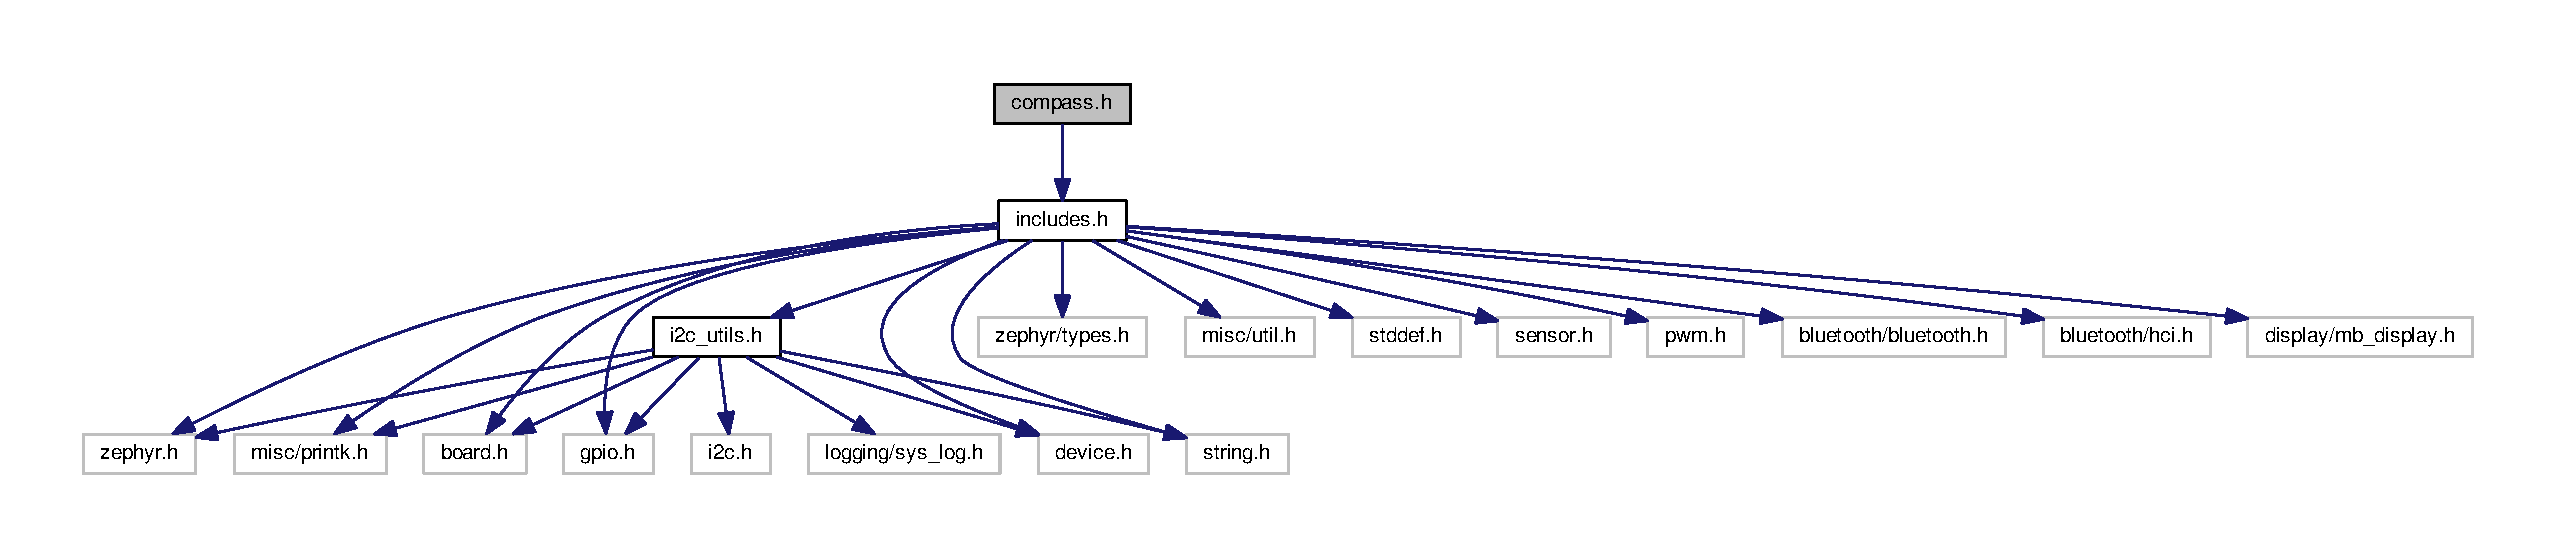
\includegraphics[width=350pt]{compass_8h__incl}
\end{center}
\end{figure}
Este grafo mostra quais arquivos estão direta ou indiretamente relacionados com este arquivo\+:\nopagebreak
\begin{figure}[H]
\begin{center}
\leavevmode
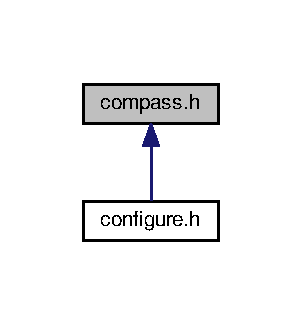
\includegraphics[width=145pt]{compass_8h__dep__incl}
\end{center}
\end{figure}
\subsection*{Definições e Macros}
\begin{DoxyCompactItemize}
\item 
\#define \hyperlink{compass_8h_a0deae345f38c0e72dd027b6c2e7c38e7}{C\+O\+M\+P\+A\+S\+S\+\_\+\+A\+D\+D\+R\+E\+SS}~0x0e
\item 
\#define \hyperlink{compass_8h_ad6ecd848e176fd228e159d1e9bf0d445}{C\+O\+M\+P\+A\+S\+S\+\_\+\+R\+E\+G\+I\+S\+T\+ER}~0x07
\item 
\#define \hyperlink{compass_8h_a7c8204e4e26f069411ac8c96ea3ad129}{C\+O\+M\+P\+A\+S\+S\+\_\+\+T\+E\+ST}~0x\+C4
\item 
\#define \hyperlink{compass_8h_aec4a4eac5b9b6a4f984b06fc1f89448e}{R\+E\+F\+R\+E\+S\+H\+\_\+\+T\+I\+M\+E\+\_\+\+C\+O\+M\+P\+A\+SS}~1000
\end{DoxyCompactItemize}
\subsection*{Funções}
\begin{DoxyCompactItemize}
\item 
void \hyperlink{compass_8h_a28af8cd17e7340de7115170728bf4915}{compass\+\_\+display} ()\hypertarget{compass_8h_a28af8cd17e7340de7115170728bf4915}{}\label{compass_8h_a28af8cd17e7340de7115170728bf4915}

\begin{DoxyCompactList}\small\item\em Função que irá mostrar na Matriz 5x5 um \char`\"{}\+T\char`\"{}. \end{DoxyCompactList}\item 
void \hyperlink{compass_8h_a9325b2f8617cef31301292bb0d30c04f}{compass\+\_\+showcase} ()\hypertarget{compass_8h_a9325b2f8617cef31301292bb0d30c04f}{}\label{compass_8h_a9325b2f8617cef31301292bb0d30c04f}

\begin{DoxyCompactList}\small\item\em Função que irá executar a funcionalidade da Bússola Implementada. \end{DoxyCompactList}\item 
void \hyperlink{compass_8h_af3422b44dd53d24518dfe42a6a485add}{init\+\_\+compass} ()\hypertarget{compass_8h_af3422b44dd53d24518dfe42a6a485add}{}\label{compass_8h_af3422b44dd53d24518dfe42a6a485add}

\begin{DoxyCompactList}\small\item\em Método que irá iniciar as variáveis responsáveis pelo bom funcionamento da Bússola. \end{DoxyCompactList}\end{DoxyCompactItemize}
\subsection*{Variáveis}
\begin{DoxyCompactItemize}
\item 
struct \hyperlink{structi2c__dev}{i2c\+\_\+dev} \hyperlink{compass_8h_a52e4a8d90dbb3179114b45e6bb717b27}{compass}\hypertarget{compass_8h_a52e4a8d90dbb3179114b45e6bb717b27}{}\label{compass_8h_a52e4a8d90dbb3179114b45e6bb717b27}

\begin{DoxyCompactList}\small\item\em Variável responsável por estabelecer a comunicação I²C com a Bússola. \end{DoxyCompactList}\end{DoxyCompactItemize}


\subsection{Descrição Detalhada}
Este arquivo contém as funções, constantes e variáveis relacionadas a funcionalidade da Bússola. 

\begin{DoxyAuthor}{Autor}
Bruno Georgevich Ferreira 
\end{DoxyAuthor}
\begin{DoxyDate}{Data}
27 May 2018 
\end{DoxyDate}


\subsection{Definições e macros}
\index{compass.\+h@{compass.\+h}!C\+O\+M\+P\+A\+S\+S\+\_\+\+A\+D\+D\+R\+E\+SS@{C\+O\+M\+P\+A\+S\+S\+\_\+\+A\+D\+D\+R\+E\+SS}}
\index{C\+O\+M\+P\+A\+S\+S\+\_\+\+A\+D\+D\+R\+E\+SS@{C\+O\+M\+P\+A\+S\+S\+\_\+\+A\+D\+D\+R\+E\+SS}!compass.\+h@{compass.\+h}}
\subsubsection[{\texorpdfstring{C\+O\+M\+P\+A\+S\+S\+\_\+\+A\+D\+D\+R\+E\+SS}{COMPASS_ADDRESS}}]{\setlength{\rightskip}{0pt plus 5cm}\#define C\+O\+M\+P\+A\+S\+S\+\_\+\+A\+D\+D\+R\+E\+SS~0x0e}\hypertarget{compass_8h_a0deae345f38c0e72dd027b6c2e7c38e7}{}\label{compass_8h_a0deae345f38c0e72dd027b6c2e7c38e7}
Endereço da Bússola \index{compass.\+h@{compass.\+h}!C\+O\+M\+P\+A\+S\+S\+\_\+\+R\+E\+G\+I\+S\+T\+ER@{C\+O\+M\+P\+A\+S\+S\+\_\+\+R\+E\+G\+I\+S\+T\+ER}}
\index{C\+O\+M\+P\+A\+S\+S\+\_\+\+R\+E\+G\+I\+S\+T\+ER@{C\+O\+M\+P\+A\+S\+S\+\_\+\+R\+E\+G\+I\+S\+T\+ER}!compass.\+h@{compass.\+h}}
\subsubsection[{\texorpdfstring{C\+O\+M\+P\+A\+S\+S\+\_\+\+R\+E\+G\+I\+S\+T\+ER}{COMPASS_REGISTER}}]{\setlength{\rightskip}{0pt plus 5cm}\#define C\+O\+M\+P\+A\+S\+S\+\_\+\+R\+E\+G\+I\+S\+T\+ER~0x07}\hypertarget{compass_8h_ad6ecd848e176fd228e159d1e9bf0d445}{}\label{compass_8h_ad6ecd848e176fd228e159d1e9bf0d445}
Registrador da Bússola \index{compass.\+h@{compass.\+h}!C\+O\+M\+P\+A\+S\+S\+\_\+\+T\+E\+ST@{C\+O\+M\+P\+A\+S\+S\+\_\+\+T\+E\+ST}}
\index{C\+O\+M\+P\+A\+S\+S\+\_\+\+T\+E\+ST@{C\+O\+M\+P\+A\+S\+S\+\_\+\+T\+E\+ST}!compass.\+h@{compass.\+h}}
\subsubsection[{\texorpdfstring{C\+O\+M\+P\+A\+S\+S\+\_\+\+T\+E\+ST}{COMPASS_TEST}}]{\setlength{\rightskip}{0pt plus 5cm}\#define C\+O\+M\+P\+A\+S\+S\+\_\+\+T\+E\+ST~0x\+C4}\hypertarget{compass_8h_a7c8204e4e26f069411ac8c96ea3ad129}{}\label{compass_8h_a7c8204e4e26f069411ac8c96ea3ad129}
Código de Teste da Bússola \index{compass.\+h@{compass.\+h}!R\+E\+F\+R\+E\+S\+H\+\_\+\+T\+I\+M\+E\+\_\+\+C\+O\+M\+P\+A\+SS@{R\+E\+F\+R\+E\+S\+H\+\_\+\+T\+I\+M\+E\+\_\+\+C\+O\+M\+P\+A\+SS}}
\index{R\+E\+F\+R\+E\+S\+H\+\_\+\+T\+I\+M\+E\+\_\+\+C\+O\+M\+P\+A\+SS@{R\+E\+F\+R\+E\+S\+H\+\_\+\+T\+I\+M\+E\+\_\+\+C\+O\+M\+P\+A\+SS}!compass.\+h@{compass.\+h}}
\subsubsection[{\texorpdfstring{R\+E\+F\+R\+E\+S\+H\+\_\+\+T\+I\+M\+E\+\_\+\+C\+O\+M\+P\+A\+SS}{REFRESH_TIME_COMPASS}}]{\setlength{\rightskip}{0pt plus 5cm}\#define R\+E\+F\+R\+E\+S\+H\+\_\+\+T\+I\+M\+E\+\_\+\+C\+O\+M\+P\+A\+SS~1000}\hypertarget{compass_8h_aec4a4eac5b9b6a4f984b06fc1f89448e}{}\label{compass_8h_aec4a4eac5b9b6a4f984b06fc1f89448e}
Tempo de Reiterção da Bússola 
\hypertarget{configure_8h}{}\section{Referência do Arquivo configure.\+h}
\label{configure_8h}\index{configure.\+h@{configure.\+h}}


Este arquivo contém as funções, constantes e variáveis responsáveis por configurar e abstrair os Sensores da Micro\+Bit.  


{\ttfamily \#include \char`\"{}includes.\+h\char`\"{}}\\*
{\ttfamily \#include \char`\"{}helloworld.\+h\char`\"{}}\\*
{\ttfamily \#include \char`\"{}temperature.\+h\char`\"{}}\\*
{\ttfamily \#include \char`\"{}accelerometer.\+h\char`\"{}}\\*
{\ttfamily \#include \char`\"{}compass.\+h\char`\"{}}\\*
{\ttfamily \#include \char`\"{}state.\+h\char`\"{}}\\*
Gráfico de dependência de inclusões para configure.\+h\+:\nopagebreak
\begin{figure}[H]
\begin{center}
\leavevmode
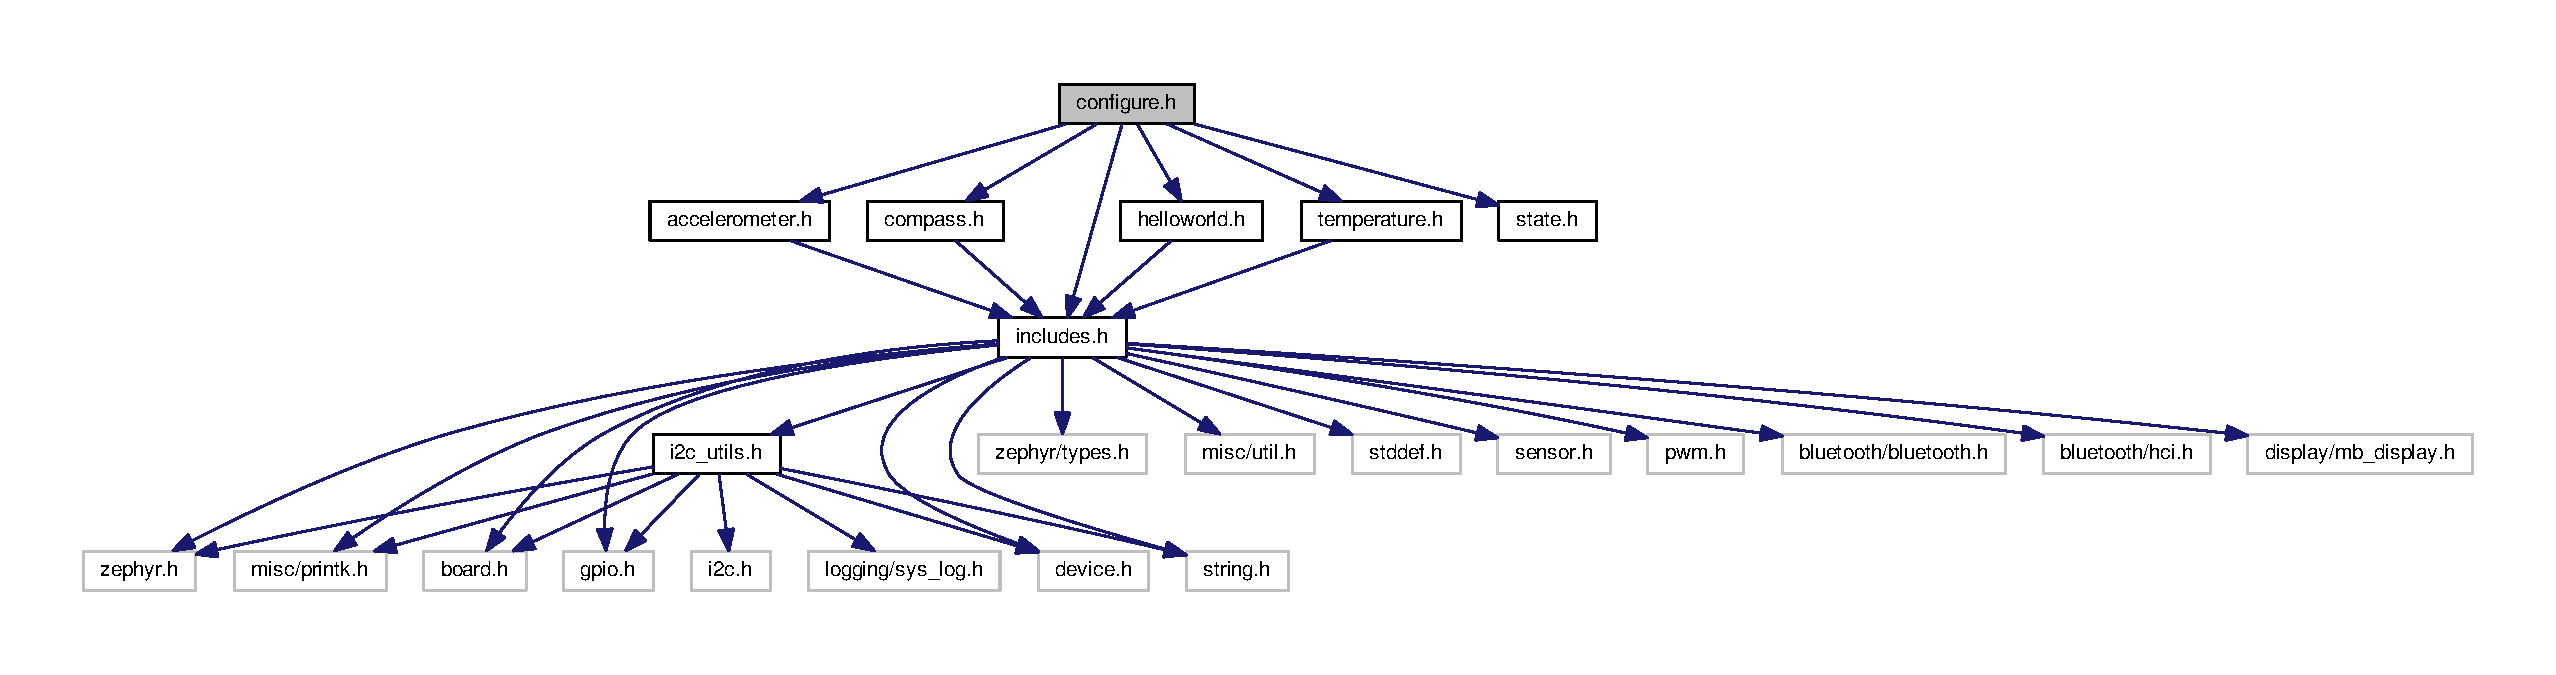
\includegraphics[width=350pt]{configure_8h__incl}
\end{center}
\end{figure}
\subsection*{Definições e Macros}
\begin{DoxyCompactItemize}
\item 
\#define \hyperlink{configure_8h_a4665ddd28964cf2d8afbcdcdb8b147e8}{P\+R\+O\+G\+R\+A\+M\+\_\+\+R\+U\+N\+S\+\_\+\+C\+O\+R\+R\+E\+C\+T\+LY}~1
\item 
\#define \hyperlink{configure_8h_a15218844bd3bc87e3ff485780c675998}{N\+O\+\_\+\+E\+R\+R\+O\+RS}~0
\item 
\#define \hyperlink{configure_8h_ad72dbcf6d0153db1b8d8a58001feed83}{D\+E\+B\+UG}
\end{DoxyCompactItemize}
\subsection*{Funções}
\begin{DoxyCompactItemize}
\item 
void \hyperlink{configure_8h_acc6cd67b731447c215f82c81fffdfa5f}{button\+\_\+pressed} (struct device $\ast$dev, struct gpio\+\_\+callback $\ast$cb, u32\+\_\+t pins)\hypertarget{configure_8h_acc6cd67b731447c215f82c81fffdfa5f}{}\label{configure_8h_acc6cd67b731447c215f82c81fffdfa5f}

\begin{DoxyCompactList}\small\item\em Função que irá identificar o botão apertado e executar a ação delegada ao mesmo. \end{DoxyCompactList}\item 
void \hyperlink{configure_8h_aa5669c257d560bbb1ae4c9eebde97efd}{configure\+\_\+buttons} (void)\hypertarget{configure_8h_aa5669c257d560bbb1ae4c9eebde97efd}{}\label{configure_8h_aa5669c257d560bbb1ae4c9eebde97efd}

\begin{DoxyCompactList}\small\item\em Função responsável por configurar os botões e seus devidos pinos e callbacks. \end{DoxyCompactList}\item 
void \hyperlink{configure_8h_ad7577ba7f06f417a019b69da8682ede5}{init\+\_\+sensors} (void)\hypertarget{configure_8h_ad7577ba7f06f417a019b69da8682ede5}{}\label{configure_8h_ad7577ba7f06f417a019b69da8682ede5}

\begin{DoxyCompactList}\small\item\em Função responsável por inicializar todos os sensores utilizados no projeto. \end{DoxyCompactList}\item 
void \hyperlink{configure_8h_aeb85c296fae392e3c75a675d66e0357a}{init\+\_\+state\+\_\+machine} (void)\hypertarget{configure_8h_aeb85c296fae392e3c75a675d66e0357a}{}\label{configure_8h_aeb85c296fae392e3c75a675d66e0357a}

\begin{DoxyCompactList}\small\item\em Função responsável por inicializar a Máquina de Estados. \end{DoxyCompactList}\end{DoxyCompactItemize}
\subsection*{Variáveis}
\begin{DoxyCompactItemize}
\item 
s64\+\_\+t \hyperlink{configure_8h_a6521179d005835fc4671d4fb5b9f31a1}{a\+\_\+timestamp}\hypertarget{configure_8h_a6521179d005835fc4671d4fb5b9f31a1}{}\label{configure_8h_a6521179d005835fc4671d4fb5b9f31a1}

\begin{DoxyCompactList}\small\item\em Variável responsável por armazenar o momento que o qual o último clique foi realizado no Botão A. \end{DoxyCompactList}\item 
s64\+\_\+t \hyperlink{configure_8h_a2244551330ffddfb615f9ef02dabf65e}{b\+\_\+timestamp}\hypertarget{configure_8h_a2244551330ffddfb615f9ef02dabf65e}{}\label{configure_8h_a2244551330ffddfb615f9ef02dabf65e}

\begin{DoxyCompactList}\small\item\em Variável responsável por armazenar o momento que o qual o último clique foi realizado no Botão B. \end{DoxyCompactList}\item 
struct \hyperlink{structstate}{state} \hyperlink{configure_8h_ada99a16d29437b18c0e931b401d452e9}{state\+\_\+machine} \mbox{[}4\mbox{]}\hypertarget{configure_8h_ada99a16d29437b18c0e931b401d452e9}{}\label{configure_8h_ada99a16d29437b18c0e931b401d452e9}

\begin{DoxyCompactList}\small\item\em Variável responsável por armazenar o estados predefinidos da Máquina de Estados. \end{DoxyCompactList}\item 
enum \hyperlink{state_8h_aa0aafed44fec19806d8f9ad834be1248}{state\+\_\+t} \hyperlink{configure_8h_a56e95103335d590a068c27e16266e1f4}{current\+\_\+state\+\_\+t}\hypertarget{configure_8h_a56e95103335d590a068c27e16266e1f4}{}\label{configure_8h_a56e95103335d590a068c27e16266e1f4}

\begin{DoxyCompactList}\small\item\em Variável responsável por referenciar o tipo do estado atual. \end{DoxyCompactList}\item 
struct \hyperlink{structstate}{state} $\ast$ \hyperlink{configure_8h_aef6ecbc1dd335d8fa9ec8fe1c051057b}{current\+\_\+state}\hypertarget{configure_8h_aef6ecbc1dd335d8fa9ec8fe1c051057b}{}\label{configure_8h_aef6ecbc1dd335d8fa9ec8fe1c051057b}

\begin{DoxyCompactList}\small\item\em Variável responsável por referenciar o estado atual. \end{DoxyCompactList}\end{DoxyCompactItemize}


\subsection{Descrição Detalhada}
Este arquivo contém as funções, constantes e variáveis responsáveis por configurar e abstrair os Sensores da Micro\+Bit. 

\begin{DoxyAuthor}{Autor}
Bruno Georgevich Ferreira 
\end{DoxyAuthor}
\begin{DoxyDate}{Data}
27 May 2018 
\end{DoxyDate}


\subsection{Definições e macros}
\index{configure.\+h@{configure.\+h}!D\+E\+B\+UG@{D\+E\+B\+UG}}
\index{D\+E\+B\+UG@{D\+E\+B\+UG}!configure.\+h@{configure.\+h}}
\subsubsection[{\texorpdfstring{D\+E\+B\+UG}{DEBUG}}]{\setlength{\rightskip}{0pt plus 5cm}\#define D\+E\+B\+UG}\hypertarget{configure_8h_ad72dbcf6d0153db1b8d8a58001feed83}{}\label{configure_8h_ad72dbcf6d0153db1b8d8a58001feed83}
Constante responsável por habilitar os printk\textquotesingle{}s do código \index{configure.\+h@{configure.\+h}!N\+O\+\_\+\+E\+R\+R\+O\+RS@{N\+O\+\_\+\+E\+R\+R\+O\+RS}}
\index{N\+O\+\_\+\+E\+R\+R\+O\+RS@{N\+O\+\_\+\+E\+R\+R\+O\+RS}!configure.\+h@{configure.\+h}}
\subsubsection[{\texorpdfstring{N\+O\+\_\+\+E\+R\+R\+O\+RS}{NO_ERRORS}}]{\setlength{\rightskip}{0pt plus 5cm}\#define N\+O\+\_\+\+E\+R\+R\+O\+RS~0}\hypertarget{configure_8h_a15218844bd3bc87e3ff485780c675998}{}\label{configure_8h_a15218844bd3bc87e3ff485780c675998}
Constante responsável por agregar legibilidade ao retorno 0 da função Main \index{configure.\+h@{configure.\+h}!P\+R\+O\+G\+R\+A\+M\+\_\+\+R\+U\+N\+S\+\_\+\+C\+O\+R\+R\+E\+C\+T\+LY@{P\+R\+O\+G\+R\+A\+M\+\_\+\+R\+U\+N\+S\+\_\+\+C\+O\+R\+R\+E\+C\+T\+LY}}
\index{P\+R\+O\+G\+R\+A\+M\+\_\+\+R\+U\+N\+S\+\_\+\+C\+O\+R\+R\+E\+C\+T\+LY@{P\+R\+O\+G\+R\+A\+M\+\_\+\+R\+U\+N\+S\+\_\+\+C\+O\+R\+R\+E\+C\+T\+LY}!configure.\+h@{configure.\+h}}
\subsubsection[{\texorpdfstring{P\+R\+O\+G\+R\+A\+M\+\_\+\+R\+U\+N\+S\+\_\+\+C\+O\+R\+R\+E\+C\+T\+LY}{PROGRAM_RUNS_CORRECTLY}}]{\setlength{\rightskip}{0pt plus 5cm}\#define P\+R\+O\+G\+R\+A\+M\+\_\+\+R\+U\+N\+S\+\_\+\+C\+O\+R\+R\+E\+C\+T\+LY~1}\hypertarget{configure_8h_a4665ddd28964cf2d8afbcdcdb8b147e8}{}\label{configure_8h_a4665ddd28964cf2d8afbcdcdb8b147e8}
Constante responsável por agregar legibilidade ao loop de iterações da execução do estado atual 
\hypertarget{helloworld_8h}{}\section{Referência do Arquivo helloworld.\+h}
\label{helloworld_8h}\index{helloworld.\+h@{helloworld.\+h}}


Este arquivo contém as funções, constantes e variáveis relacionadas a funcionalidade Hello\+World.  


{\ttfamily \#include \char`\"{}includes.\+h\char`\"{}}\\*
Gráfico de dependência de inclusões para helloworld.\+h\+:\nopagebreak
\begin{figure}[H]
\begin{center}
\leavevmode
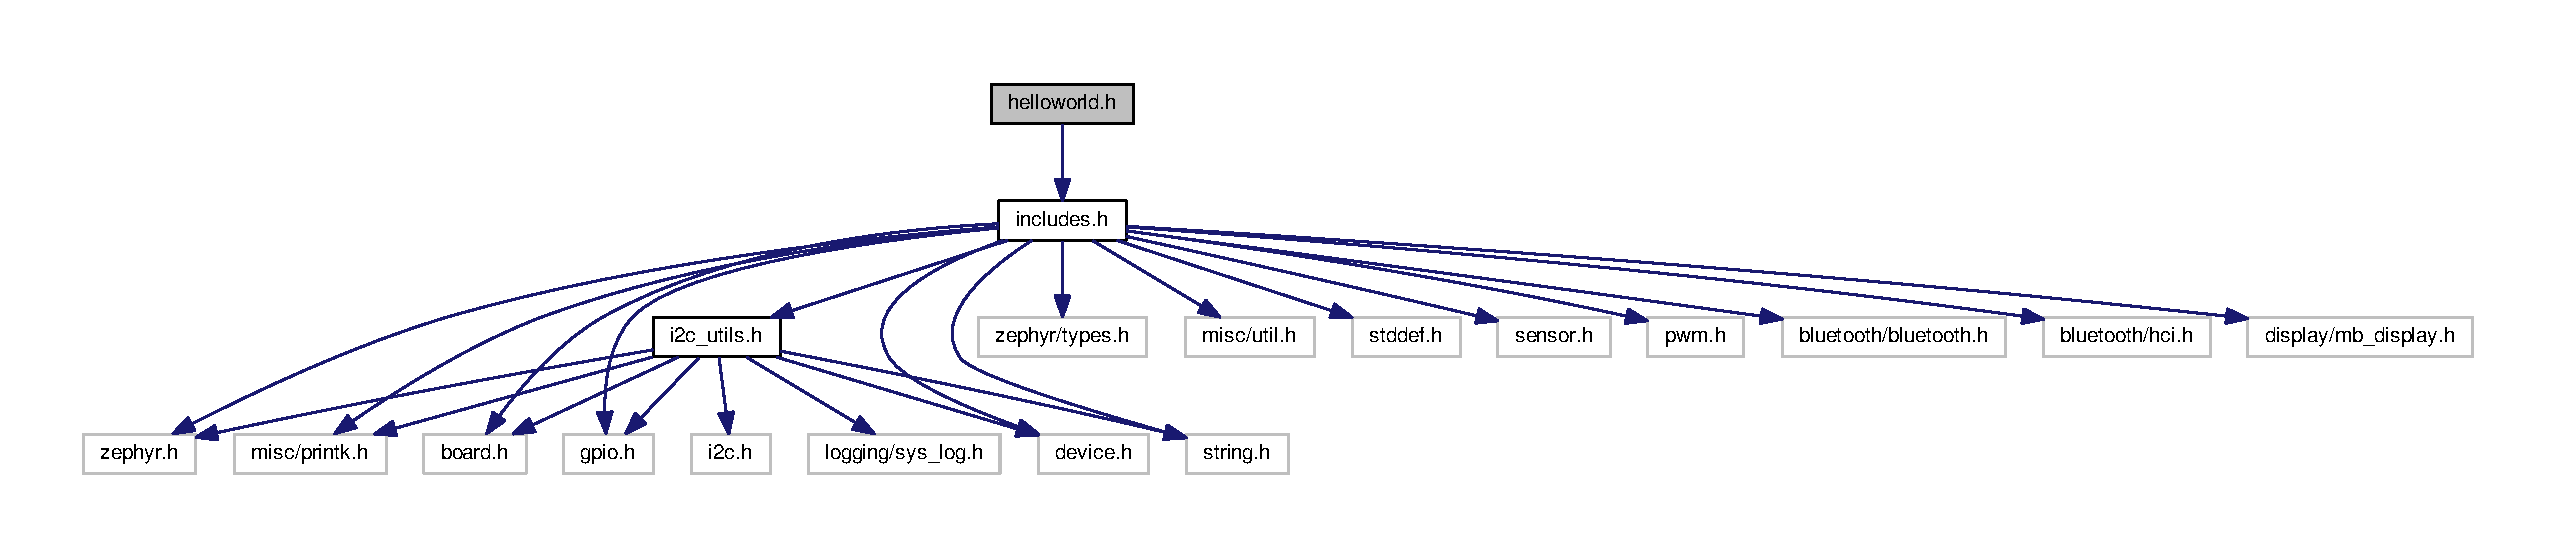
\includegraphics[width=350pt]{helloworld_8h__incl}
\end{center}
\end{figure}
Este grafo mostra quais arquivos estão direta ou indiretamente relacionados com este arquivo\+:\nopagebreak
\begin{figure}[H]
\begin{center}
\leavevmode
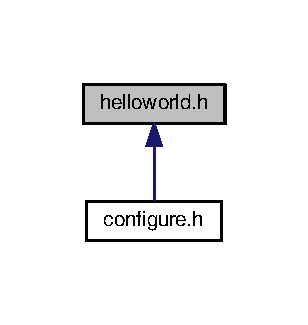
\includegraphics[width=148pt]{helloworld_8h__dep__incl}
\end{center}
\end{figure}
\subsection*{Definições e Macros}
\begin{DoxyCompactItemize}
\item 
\#define \hyperlink{helloworld_8h_a640c70923109c4da08dc8d463ce23e1a}{R\+E\+F\+R\+E\+S\+H\+\_\+\+T\+I\+M\+E\+\_\+\+H\+E\+L\+L\+O\+W\+O\+R\+LD}~1000
\end{DoxyCompactItemize}
\subsection*{Funções}
\begin{DoxyCompactItemize}
\item 
void \hyperlink{helloworld_8h_a431f6b4e2319fd239c94c6477b3df781}{helloworld\+\_\+showcase} ()\hypertarget{helloworld_8h_a431f6b4e2319fd239c94c6477b3df781}{}\label{helloworld_8h_a431f6b4e2319fd239c94c6477b3df781}

\begin{DoxyCompactList}\small\item\em Função que irá executar a funcionalidade Hello\+World Implementada. \end{DoxyCompactList}\end{DoxyCompactItemize}


\subsection{Descrição Detalhada}
Este arquivo contém as funções, constantes e variáveis relacionadas a funcionalidade Hello\+World. 

\begin{DoxyAuthor}{Autor}
Bruno Georgevich Ferreira 
\end{DoxyAuthor}
\begin{DoxyDate}{Data}
27 May 2018 
\end{DoxyDate}


\subsection{Definições e macros}
\index{helloworld.\+h@{helloworld.\+h}!R\+E\+F\+R\+E\+S\+H\+\_\+\+T\+I\+M\+E\+\_\+\+H\+E\+L\+L\+O\+W\+O\+R\+LD@{R\+E\+F\+R\+E\+S\+H\+\_\+\+T\+I\+M\+E\+\_\+\+H\+E\+L\+L\+O\+W\+O\+R\+LD}}
\index{R\+E\+F\+R\+E\+S\+H\+\_\+\+T\+I\+M\+E\+\_\+\+H\+E\+L\+L\+O\+W\+O\+R\+LD@{R\+E\+F\+R\+E\+S\+H\+\_\+\+T\+I\+M\+E\+\_\+\+H\+E\+L\+L\+O\+W\+O\+R\+LD}!helloworld.\+h@{helloworld.\+h}}
\subsubsection[{\texorpdfstring{R\+E\+F\+R\+E\+S\+H\+\_\+\+T\+I\+M\+E\+\_\+\+H\+E\+L\+L\+O\+W\+O\+R\+LD}{REFRESH_TIME_HELLOWORLD}}]{\setlength{\rightskip}{0pt plus 5cm}\#define R\+E\+F\+R\+E\+S\+H\+\_\+\+T\+I\+M\+E\+\_\+\+H\+E\+L\+L\+O\+W\+O\+R\+LD~1000}\hypertarget{helloworld_8h_a640c70923109c4da08dc8d463ce23e1a}{}\label{helloworld_8h_a640c70923109c4da08dc8d463ce23e1a}
Tempo de Reiterção do Hello\+World 
\hypertarget{i2c__utils_8h}{}\section{Referência do Arquivo i2c\+\_\+utils.\+h}
\label{i2c__utils_8h}\index{i2c\+\_\+utils.\+h@{i2c\+\_\+utils.\+h}}


Este arquivo contém as constantes, funções e variáveis relacionadas a Comunicação I²C.  


{\ttfamily \#include $<$zephyr.\+h$>$}\\*
{\ttfamily \#include $<$misc/printk.\+h$>$}\\*
{\ttfamily \#include $<$board.\+h$>$}\\*
{\ttfamily \#include $<$gpio.\+h$>$}\\*
{\ttfamily \#include $<$device.\+h$>$}\\*
{\ttfamily \#include $<$i2c.\+h$>$}\\*
{\ttfamily \#include $<$string.\+h$>$}\\*
{\ttfamily \#include $<$logging/sys\+\_\+log.\+h$>$}\\*
Gráfico de dependência de inclusões para i2c\+\_\+utils.\+h\+:\nopagebreak
\begin{figure}[H]
\begin{center}
\leavevmode
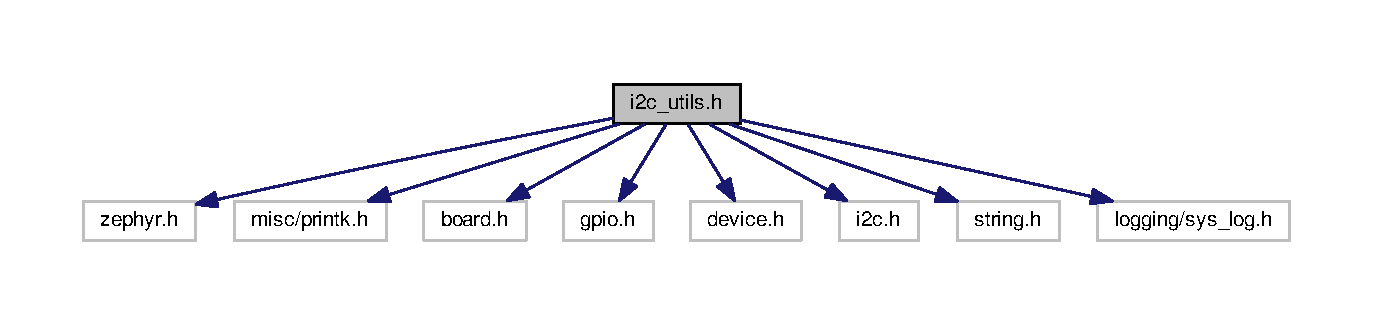
\includegraphics[width=350pt]{i2c__utils_8h__incl}
\end{center}
\end{figure}
Este grafo mostra quais arquivos estão direta ou indiretamente relacionados com este arquivo\+:\nopagebreak
\begin{figure}[H]
\begin{center}
\leavevmode
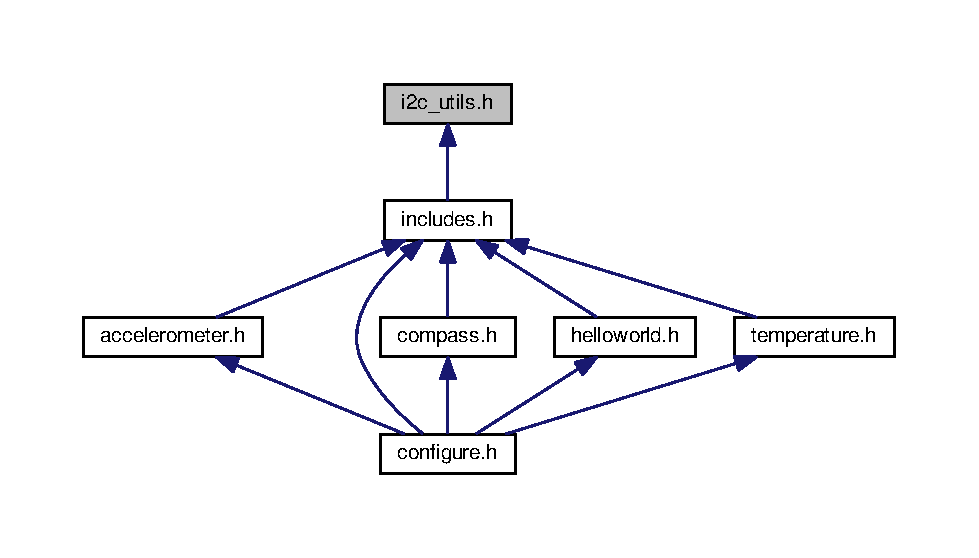
\includegraphics[width=350pt]{i2c__utils_8h__dep__incl}
\end{center}
\end{figure}
\subsection*{Estruturas de Dados}
\begin{DoxyCompactItemize}
\item 
struct \hyperlink{structi2c__dev}{i2c\+\_\+dev}
\end{DoxyCompactItemize}
\subsection*{Definições e Macros}
\begin{DoxyCompactItemize}
\item 
\#define {\bfseries S\+Y\+S\+\_\+\+L\+O\+G\+\_\+\+D\+O\+M\+A\+IN}~\char`\"{}P\+R\+O\+J\+E\+CT\char`\"{}\hypertarget{i2c__utils_8h_ac5b2cb2d6ae6b5526953a00f765a23e4}{}\label{i2c__utils_8h_ac5b2cb2d6ae6b5526953a00f765a23e4}

\item 
\#define {\bfseries I2\+C\+\_\+\+D\+E\+V\+I\+C\+E\+\_\+\+N\+A\+M\+E\+\_\+\+L\+E\+N\+G\+TH}~10\hypertarget{i2c__utils_8h_a48e1e64a2a8c3e1e1df44760d2a73eaa}{}\label{i2c__utils_8h_a48e1e64a2a8c3e1e1df44760d2a73eaa}

\end{DoxyCompactItemize}
\subsection*{Funções}
\begin{DoxyCompactItemize}
\item 
int {\bfseries i2c\+\_\+util\+\_\+dev\+\_\+init} (struct \hyperlink{structi2c__dev}{i2c\+\_\+dev} $\ast$\hyperlink{structi2c__dev}{i2c\+\_\+dev}, u16\+\_\+t addr, const char $\ast$name, u8\+\_\+t reg\+\_\+test, u8\+\_\+t reg\+\_\+test\+\_\+expected\+\_\+val)\hypertarget{i2c__utils_8h_a94dc84189a2c77ce509621dc4adb8150}{}\label{i2c__utils_8h_a94dc84189a2c77ce509621dc4adb8150}

\item 
int {\bfseries i2c\+\_\+util\+\_\+write\+\_\+bytes} (struct \hyperlink{structi2c__dev}{i2c\+\_\+dev} $\ast$\hyperlink{structi2c__dev}{i2c\+\_\+dev}, u8\+\_\+t reg, u8\+\_\+t $\ast$data, u32\+\_\+t num\+\_\+bytes)\hypertarget{i2c__utils_8h_a9bdf91cfea8b14d68bc7d8819e7ba742}{}\label{i2c__utils_8h_a9bdf91cfea8b14d68bc7d8819e7ba742}

\item 
int {\bfseries i2c\+\_\+util\+\_\+read\+\_\+bytes} (struct \hyperlink{structi2c__dev}{i2c\+\_\+dev} $\ast$\hyperlink{structi2c__dev}{i2c\+\_\+dev}, u8\+\_\+t reg, u8\+\_\+t $\ast$data, u32\+\_\+t num\+\_\+bytes)\hypertarget{i2c__utils_8h_a7510a339f80427d63e309fd8b6613ce7}{}\label{i2c__utils_8h_a7510a339f80427d63e309fd8b6613ce7}

\item 
int {\bfseries i2c\+\_\+util\+\_\+test\+\_\+connection} (struct \hyperlink{structi2c__dev}{i2c\+\_\+dev} $\ast$\hyperlink{structi2c__dev}{i2c\+\_\+dev})\hypertarget{i2c__utils_8h_a7879cbd3e3c4f64e2b36ef77aaf0ec85}{}\label{i2c__utils_8h_a7879cbd3e3c4f64e2b36ef77aaf0ec85}

\end{DoxyCompactItemize}


\subsection{Descrição Detalhada}
Este arquivo contém as constantes, funções e variáveis relacionadas a Comunicação I²C. 

\begin{DoxyAuthor}{Autor}
Zephyr 
\end{DoxyAuthor}

\hypertarget{includes_8h}{}\section{Referência do Arquivo includes.\+h}
\label{includes_8h}\index{includes.\+h@{includes.\+h}}


Este arquivo contém todas as bibliotecas necessárias para os arquivos .h.  


{\ttfamily \#include $<$zephyr.\+h$>$}\\*
{\ttfamily \#include $<$zephyr/types.\+h$>$}\\*
{\ttfamily \#include $<$misc/printk.\+h$>$}\\*
{\ttfamily \#include $<$misc/util.\+h$>$}\\*
{\ttfamily \#include $<$stddef.\+h$>$}\\*
{\ttfamily \#include $<$board.\+h$>$}\\*
{\ttfamily \#include $<$gpio.\+h$>$}\\*
{\ttfamily \#include $<$device.\+h$>$}\\*
{\ttfamily \#include $<$sensor.\+h$>$}\\*
{\ttfamily \#include $<$string.\+h$>$}\\*
{\ttfamily \#include $<$pwm.\+h$>$}\\*
{\ttfamily \#include $<$bluetooth/bluetooth.\+h$>$}\\*
{\ttfamily \#include $<$bluetooth/hci.\+h$>$}\\*
{\ttfamily \#include $<$display/mb\+\_\+display.\+h$>$}\\*
{\ttfamily \#include \char`\"{}i2c\+\_\+utils.\+h\char`\"{}}\\*
Gráfico de dependência de inclusões para includes.\+h\+:\nopagebreak
\begin{figure}[H]
\begin{center}
\leavevmode
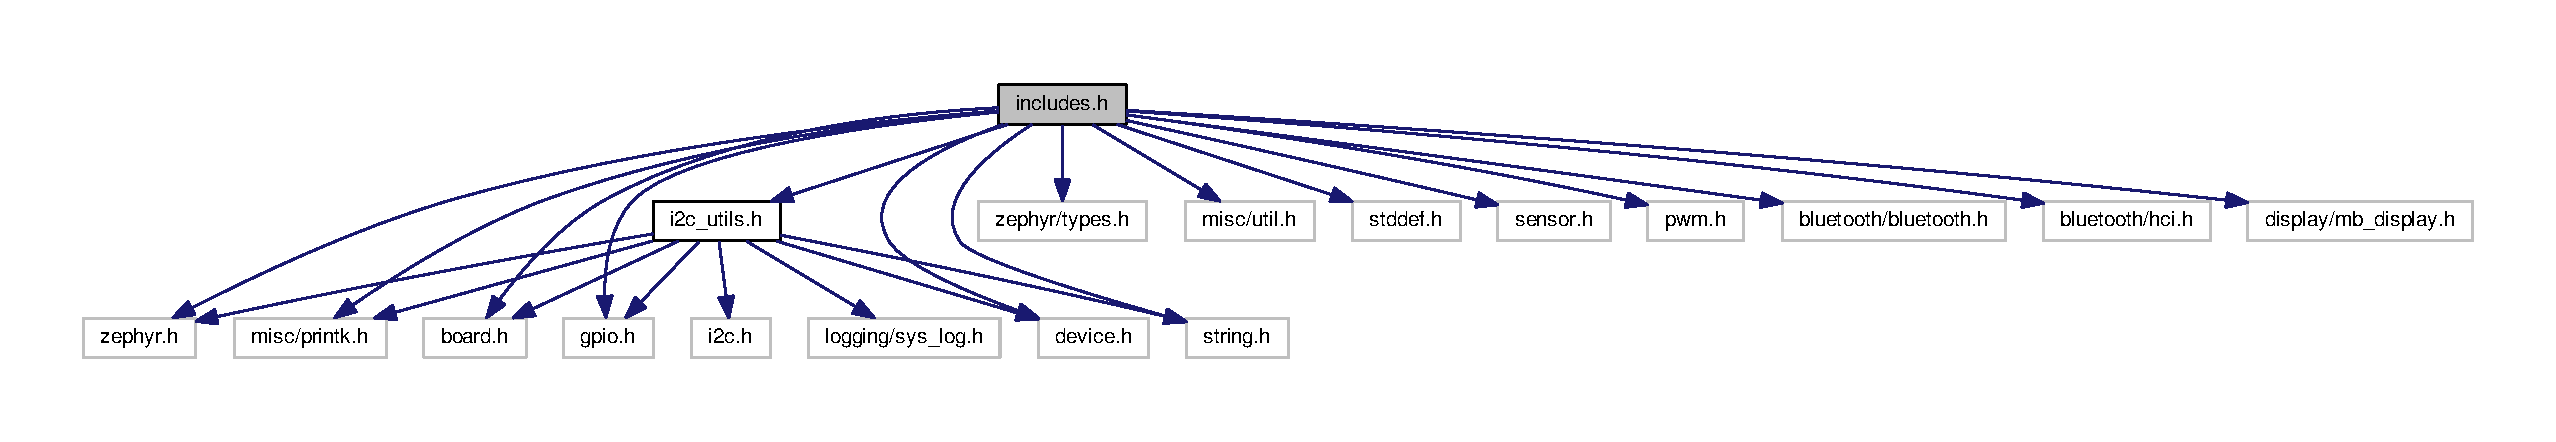
\includegraphics[width=350pt]{includes_8h__incl}
\end{center}
\end{figure}
Este grafo mostra quais arquivos estão direta ou indiretamente relacionados com este arquivo\+:\nopagebreak
\begin{figure}[H]
\begin{center}
\leavevmode
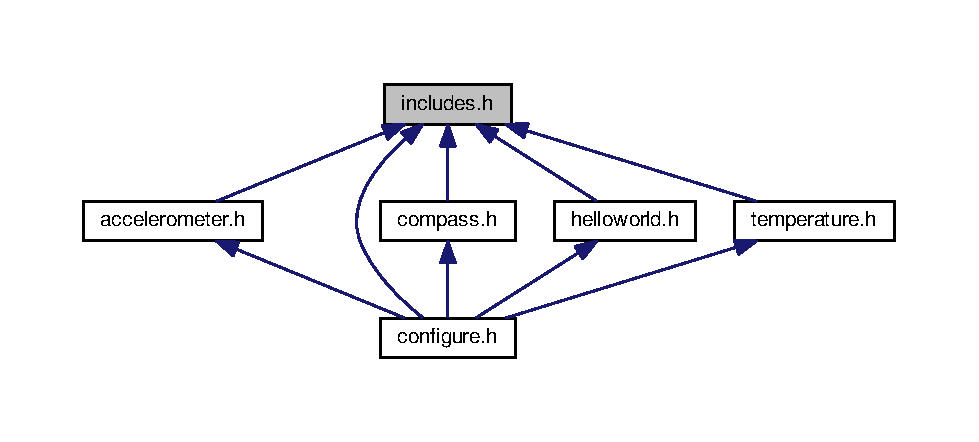
\includegraphics[width=350pt]{includes_8h__dep__incl}
\end{center}
\end{figure}


\subsection{Descrição Detalhada}
Este arquivo contém todas as bibliotecas necessárias para os arquivos .h. 

\begin{DoxyAuthor}{Autor}
Bruno Georgevich Ferreira 
\end{DoxyAuthor}
\begin{DoxyDate}{Data}
27 May 2018 
\end{DoxyDate}

\hypertarget{state_8h}{}\section{Referência do Arquivo state.\+h}
\label{state_8h}\index{state.\+h@{state.\+h}}


Este arquivo contém as constantes e variáveis relacionadas a Máquina de Estados.  


Este grafo mostra quais arquivos estão direta ou indiretamente relacionados com este arquivo\+:\nopagebreak
\begin{figure}[H]
\begin{center}
\leavevmode
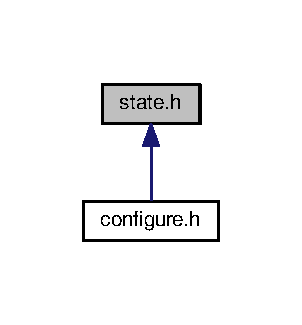
\includegraphics[width=145pt]{state_8h__dep__incl}
\end{center}
\end{figure}
\subsection*{Estruturas de Dados}
\begin{DoxyCompactItemize}
\item 
struct \hyperlink{structstate}{state}
\begin{DoxyCompactList}\small\item\em Struct que modela o formato de um estado da Máquina de Estados. \end{DoxyCompactList}\end{DoxyCompactItemize}
\subsection*{Enumerações}
\begin{DoxyCompactItemize}
\item 
enum \hyperlink{state_8h_aa0aafed44fec19806d8f9ad834be1248}{state\+\_\+t} \{ \hyperlink{state_8h_aa0aafed44fec19806d8f9ad834be1248a11d8681f1579abb9130b1d4d8cc13a44}{H\+E\+L\+L\+O\+W\+O\+R\+LD}, 
\hyperlink{state_8h_aa0aafed44fec19806d8f9ad834be1248ac4ae6787ff1d8b2d1cf0ae9aa696e56c}{T\+E\+M\+P\+E\+R\+A\+T\+U\+RE}, 
\hyperlink{state_8h_aa0aafed44fec19806d8f9ad834be1248ae2861f6a10788d276d24806767e6a378}{A\+C\+C\+E\+L\+E\+T\+O\+M\+E\+T\+ER}, 
\hyperlink{state_8h_aa0aafed44fec19806d8f9ad834be1248a7bcb838d6da81cce9b69c4ebfd47bbd6}{M\+A\+G\+N\+E\+T\+O\+M\+E\+T\+ER}
 \}\begin{DoxyCompactList}\small\item\em Enum responsável por definir os estados da Máquina de Estados. \end{DoxyCompactList}
\end{DoxyCompactItemize}


\subsection{Descrição Detalhada}
Este arquivo contém as constantes e variáveis relacionadas a Máquina de Estados. 

\begin{DoxyAuthor}{Autor}
Bruno Georgevich Ferreira 
\end{DoxyAuthor}
\begin{DoxyDate}{Data}
27 May 2018 
\end{DoxyDate}


\subsection{Enumerações}
\index{state.\+h@{state.\+h}!state\+\_\+t@{state\+\_\+t}}
\index{state\+\_\+t@{state\+\_\+t}!state.\+h@{state.\+h}}
\subsubsection[{\texorpdfstring{state\+\_\+t}{state_t}}]{\setlength{\rightskip}{0pt plus 5cm}enum {\bf state\+\_\+t}}\hypertarget{state_8h_aa0aafed44fec19806d8f9ad834be1248}{}\label{state_8h_aa0aafed44fec19806d8f9ad834be1248}


Enum responsável por definir os estados da Máquina de Estados. 

\begin{Desc}
\item[Valores de enumerações]\par
\begin{description}
\index{H\+E\+L\+L\+O\+W\+O\+R\+LD@{H\+E\+L\+L\+O\+W\+O\+R\+LD}!state.\+h@{state.\+h}}\index{state.\+h@{state.\+h}!H\+E\+L\+L\+O\+W\+O\+R\+LD@{H\+E\+L\+L\+O\+W\+O\+R\+LD}}\item[{\em 
H\+E\+L\+L\+O\+W\+O\+R\+LD\hypertarget{state_8h_aa0aafed44fec19806d8f9ad834be1248a11d8681f1579abb9130b1d4d8cc13a44}{}\label{state_8h_aa0aafed44fec19806d8f9ad834be1248a11d8681f1579abb9130b1d4d8cc13a44}
}]Estado 1 \index{T\+E\+M\+P\+E\+R\+A\+T\+U\+RE@{T\+E\+M\+P\+E\+R\+A\+T\+U\+RE}!state.\+h@{state.\+h}}\index{state.\+h@{state.\+h}!T\+E\+M\+P\+E\+R\+A\+T\+U\+RE@{T\+E\+M\+P\+E\+R\+A\+T\+U\+RE}}\item[{\em 
T\+E\+M\+P\+E\+R\+A\+T\+U\+RE\hypertarget{state_8h_aa0aafed44fec19806d8f9ad834be1248ac4ae6787ff1d8b2d1cf0ae9aa696e56c}{}\label{state_8h_aa0aafed44fec19806d8f9ad834be1248ac4ae6787ff1d8b2d1cf0ae9aa696e56c}
}]Estado 2 \index{A\+C\+C\+E\+L\+E\+T\+O\+M\+E\+T\+ER@{A\+C\+C\+E\+L\+E\+T\+O\+M\+E\+T\+ER}!state.\+h@{state.\+h}}\index{state.\+h@{state.\+h}!A\+C\+C\+E\+L\+E\+T\+O\+M\+E\+T\+ER@{A\+C\+C\+E\+L\+E\+T\+O\+M\+E\+T\+ER}}\item[{\em 
A\+C\+C\+E\+L\+E\+T\+O\+M\+E\+T\+ER\hypertarget{state_8h_aa0aafed44fec19806d8f9ad834be1248ae2861f6a10788d276d24806767e6a378}{}\label{state_8h_aa0aafed44fec19806d8f9ad834be1248ae2861f6a10788d276d24806767e6a378}
}]Estado 3 \index{M\+A\+G\+N\+E\+T\+O\+M\+E\+T\+ER@{M\+A\+G\+N\+E\+T\+O\+M\+E\+T\+ER}!state.\+h@{state.\+h}}\index{state.\+h@{state.\+h}!M\+A\+G\+N\+E\+T\+O\+M\+E\+T\+ER@{M\+A\+G\+N\+E\+T\+O\+M\+E\+T\+ER}}\item[{\em 
M\+A\+G\+N\+E\+T\+O\+M\+E\+T\+ER\hypertarget{state_8h_aa0aafed44fec19806d8f9ad834be1248a7bcb838d6da81cce9b69c4ebfd47bbd6}{}\label{state_8h_aa0aafed44fec19806d8f9ad834be1248a7bcb838d6da81cce9b69c4ebfd47bbd6}
}]Estado 4 \end{description}
\end{Desc}

\hypertarget{temperature_8h}{}\section{Referência do Arquivo temperature.\+h}
\label{temperature_8h}\index{temperature.\+h@{temperature.\+h}}


Este arquivo contém as funções, constantes e variáveis relacionadas a funcionalidade do Sensor de Temperatura.  


{\ttfamily \#include \char`\"{}includes.\+h\char`\"{}}\\*
Gráfico de dependência de inclusões para temperature.\+h\+:\nopagebreak
\begin{figure}[H]
\begin{center}
\leavevmode
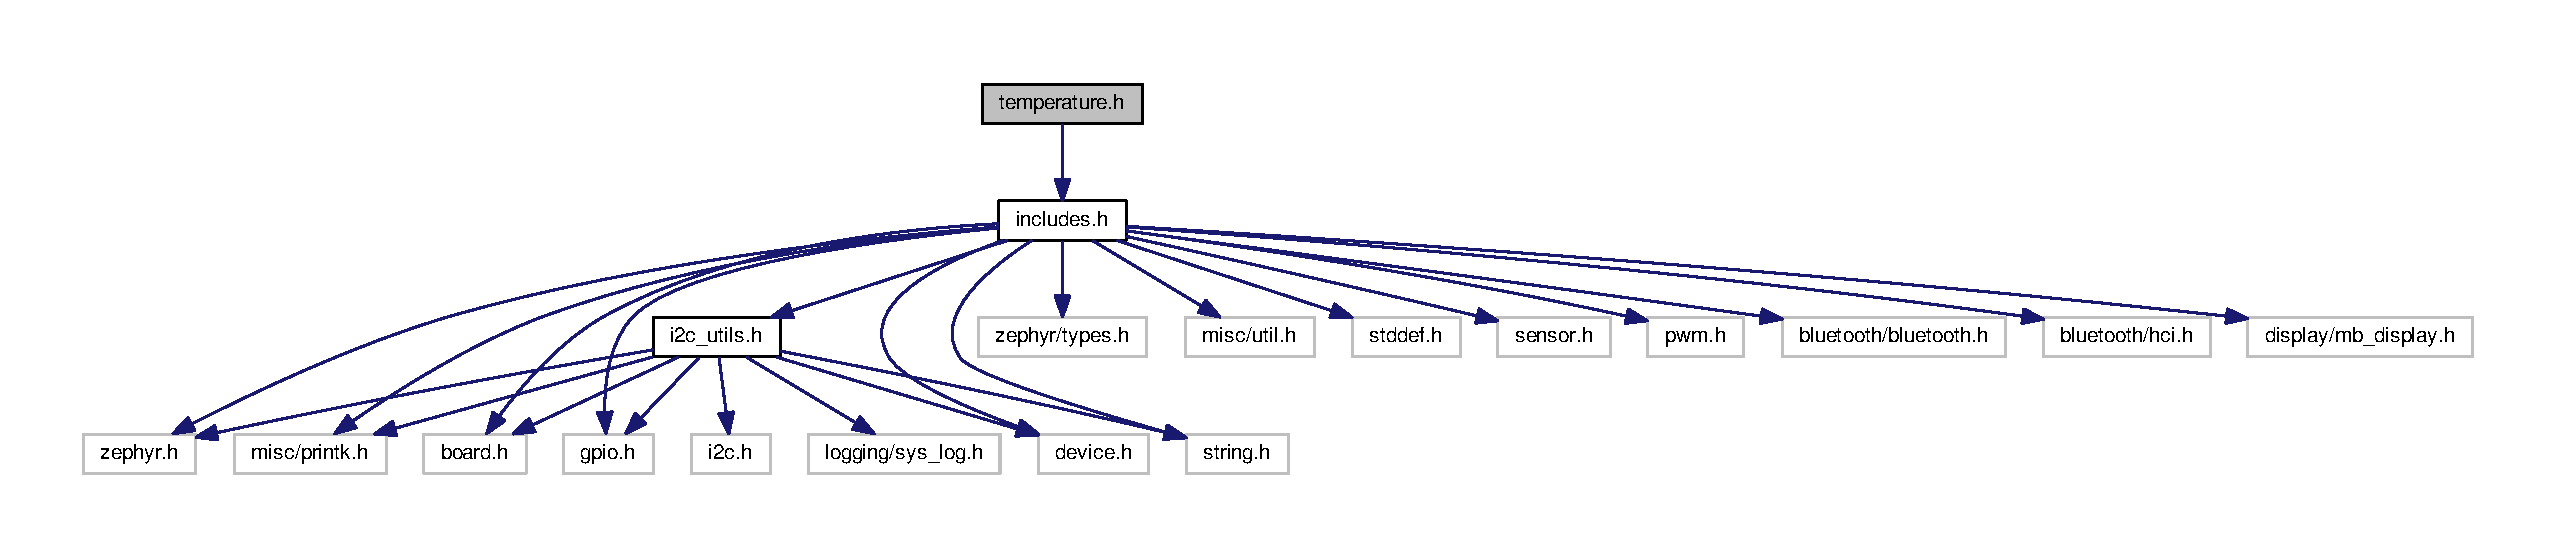
\includegraphics[width=350pt]{temperature_8h__incl}
\end{center}
\end{figure}
Este grafo mostra quais arquivos estão direta ou indiretamente relacionados com este arquivo\+:\nopagebreak
\begin{figure}[H]
\begin{center}
\leavevmode
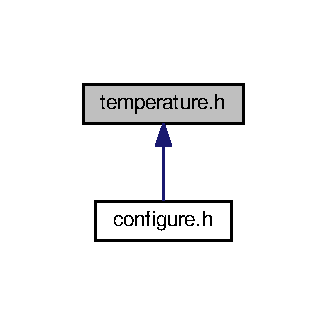
\includegraphics[width=157pt]{temperature_8h__dep__incl}
\end{center}
\end{figure}
\subsection*{Funções}
\begin{DoxyCompactItemize}
\item 
void \hyperlink{temperature_8h_a8193180919245b811d1f675fe31b114e}{temperature\+\_\+showcase} ()\hypertarget{temperature_8h_a8193180919245b811d1f675fe31b114e}{}\label{temperature_8h_a8193180919245b811d1f675fe31b114e}

\begin{DoxyCompactList}\small\item\em Função que irá executar a funcionalidade do Sensor de Temperatura Implementada. \end{DoxyCompactList}\item 
void \hyperlink{temperature_8h_aab57ff9b65744deba2a43551cc3ddd37}{init\+\_\+temperature\+\_\+sensor} ()\hypertarget{temperature_8h_aab57ff9b65744deba2a43551cc3ddd37}{}\label{temperature_8h_aab57ff9b65744deba2a43551cc3ddd37}

\begin{DoxyCompactList}\small\item\em Função que irá iniciar as variáveis responsáveis pelo bom funcionamento do Sensor de Temperatura. \end{DoxyCompactList}\end{DoxyCompactItemize}
\subsection*{Variáveis}
\begin{DoxyCompactItemize}
\item 
struct device $\ast$ \hyperlink{temperature_8h_ae7e81fbdb71af078a0c597c4424242fd}{temperature\+\_\+sensor}\hypertarget{temperature_8h_ae7e81fbdb71af078a0c597c4424242fd}{}\label{temperature_8h_ae7e81fbdb71af078a0c597c4424242fd}

\begin{DoxyCompactList}\small\item\em Variável responsável por abstrair a comunicação com o Sensor de Temperatura. \end{DoxyCompactList}\end{DoxyCompactItemize}


\subsection{Descrição Detalhada}
Este arquivo contém as funções, constantes e variáveis relacionadas a funcionalidade do Sensor de Temperatura. 

\begin{DoxyAuthor}{Autor}
Bruno Georgevich Ferreira 
\end{DoxyAuthor}
\begin{DoxyDate}{Data}
27 May 2018 
\end{DoxyDate}

%--- End generated contents ---

% Index
\backmatter
\newpage
\phantomsection
\clearemptydoublepage
\addcontentsline{toc}{chapter}{Índice}
\printindex

\end{document}
